\documentclass[11pt]{article}

\usepackage[margin=1in]{geometry}
\usepackage{graphicx}
\usepackage{float}
\usepackage{placeins}
\usepackage{booktabs}
\usepackage{amsmath,amssymb}
\usepackage{amsthm}
\usepackage{xcolor}
\usepackage{caption}
\usepackage{multirow}
\usepackage[colorlinks=true,linkcolor=blue,citecolor=blue,urlcolor=blue]{hyperref}

% float placement: the paper is figure-dense, so let floats fill more of a page
\renewcommand{\topfraction}{0.92}
\renewcommand{\bottomfraction}{0.85}
\renewcommand{\textfraction}{0.06}
\renewcommand{\floatpagefraction}{0.7}
\setcounter{topnumber}{3}
\setcounter{bottomnumber}{2}
\setcounter{totalnumber}{4}

\graphicspath{{figures/}}
\captionsetup{font=small,labelfont=bf}

\theoremstyle{plain}
\newtheorem{hypothesis}{Hypothesis}
\newtheorem{proposition}{Proposition}
\newcommand{\best}[1]{\textbf{#1}}

\title{\bfseries Mnemos-DNA: Gated Delta-Rule Linear Attention\\
with $k$-mer Fast-Weight Memory for Edge-Scale DNA Modeling}

\author{Akshat Balyan}
\date{September 10, 2026}

\begin{document}
\maketitle

\begingroup
\renewcommand\thefootnote{}\footnotetext{Code and evaluation harness:
\url{https://github.com/B4K2/Mnemos-DNA}. Pretrained checkpoints (all four arms):
\url{https://huggingface.co/B4K2xx/Mnemos-DNA}.}\endgroup

\begin{abstract}
Gated delta-rule linear attention (Kimi Delta Attention, KDA) has been validated on natural
language but, to our knowledge, never on genomic sequence modeling, where the dominant
long-context architectures are implicit convolutions (HyenaDNA) and selective state-space models
(Caduceus). We study it at a deliberately chosen operating point: \textbf{extremely low-parameter,
edge-scale DNA language models} --- $\sim$2.3M parameters, one 8\,GB consumer GPU, megabase
context --- a regime that matters on its own terms for deployment on commodity and field hardware,
and that makes single-axis architectural ablation affordable enough to run to completion. We
pretrain a family of character-level KDA models on the human reference genome (GRCh38) at a
131{,}072\,bp training context and ablate two additions: a per-$k$-mer \emph{fast-weight memory}
that attacks the finite-state recall bound of delta-rule recurrences (\textbf{Mnemos-DNA}; arm ID D06), and a coupled
prototype adding one windowed local-attention layer together with a sequence-length curriculum
(\textbf{Mnemos-DNA-C}; arm ID D07). Findings. (i)~\textbf{At this state capacity the recall bound is not a distant cliff but a wall at
distance zero}: on a repeat-copy probe over real hg38 background, a fully matched pure-KDA
control (a $32\times32$ per-head state) shows no measurable exact recall at \emph{any} distance
($\le 0.02$ nats at 64\,bp, zero beyond), and a windowed-local-attention hybrid without the
memory is indistinguishable from it; the $k$-mer fast-weight memory converts this to
0.53--0.87 nats of copy advantage sustained to 64\,kbp --- degrading by only $\approx$0.04 nats
per point substitution planted in the repeat, so the mechanism survives SNP-level divergence ---
for $\sim$3\% more parameters, a $\approx$2$\times$ prefill-throughput cost, and a 4096$\times$
larger recurrent inference state, both of which we account for explicitly.
(ii)~\textbf{The address space is used, but unevenly}: in a 131\,kbp window 63.1\%
of the $4^8$ slots are ever written against 86.5\% under a uniform-sequence null, with 68.5\% of
writes colliding and one slot (poly-T) taking 234; we give the delta rule's exact behaviour under
such repeated writes. (iii)~\textbf{Ultra-long fixed pretraining damages sub-kilobase grammar,
and neither of our patches repairs it}: under one matched fine-tuning protocol, pretrained
Mnemos-DNA reaches 0.740 on splice sites where a randomly initialized copy of itself reaches
0.832, and Mnemos-DNA-C's window-plus-curriculum leaves the gap intact (0.733); the same
control applied to the released 1M-context HyenaDNA checkpoint shows the same signature
(pretrained 0.737 vs.\ random-init $0.781\pm0.009$ on splice donors), so the effect is not
specific to delta-rule architectures.
(iv)~\textbf{Fine-tuned architecture comparisons are protocol-fragile}: we show that letting the
pooling head, epoch budget and training-set caps vary between arms --- drift that arises
naturally in any long-running study --- produces spurious cross-arm effects of up to 30 accuracy
points, an order of magnitude larger than any true architecture effect we measure; under one
frozen protocol with 2--3 fine-tuning seeds, the arms differ by $\le$1 point on every suite
mean. (v)~\textbf{Perplexity is silent on all of it}: the arms sit within 0.01 nats/base of one
another while the recall probe separates them by 0.6 nats and the random-init control exposes a
9-point fine-tuning gap. Every comparison to released baseline checkpoints (HyenaDNA, Caduceus
--- $\sim$3$\times$ our parameter count but orders of magnitude more pretraining compute) is
labelled as a deployment-feasibility comparison of artifacts, not architectures.
\end{abstract}

\section{Introduction}\label{sec:intro}

DNA foundation models face a context problem that natural-language models do not: regulatory
interactions span hundreds of kilobases, yet single-nucleotide resolution matters, so a sequence
of interest is routinely $10^5$--$10^6$ tokens long. The two families that dominate this regime
--- HyenaDNA's implicit long convolutions~\cite{nguyen2023hyenadna} and the Mamba-based
Caduceus~\cite{schiff2024caduceus} --- replace quadratic attention with sub-quadratic mixers. A
third family, \emph{gated delta-rule linear attention} (Gated DeltaNet~\cite{yang2025gated}, Kimi
Delta Attention~\cite{kimilinear2025}), has strong natural-language results but no published
genomic evaluation. Its defining weakness is also its most interesting property for genomics: the
recurrent state is a fixed $d\times d$ matrix, so exact recall of a distant motif is
information-theoretically bounded, a recall--capacity trade-off formalized in prior
work~\cite{arora2023zoology}. Genomes, full of near-exact repeats whose \emph{differences} carry
the signal, should be a stress test for exactly this bound.

\paragraph{Edge-scale is the design objective, not a constraint we apologize for.}
This work targets an operating point of $\sim$2.3M parameters and a single 8\,GB consumer GPU
(RTX~5060 Laptop). That choice is deliberate and has two independent justifications. First, it is
a deployment regime with its own demand: sequencing-adjacent analysis increasingly runs on
laptops, clinic workstations, and field devices, where a model that processes a megabase window
in 5.6\,GB is usable and a released checkpoint that goes out of memory at 512\,kbp is not.
Second, it is the regime in which a full single-axis ablation is actually finishable: every arm
here is pretrained from scratch on a matched tokenizer, matched data order and matched token
budget, which is what licenses attributing a difference to the one ingredient that changed.
Large-scale reports rarely can, because they bundle architecture, budget, and data changes.
We accordingly do not claim that findings here transfer to 100M+ scale, and we mark the places
where the $d_{\text{model}}{=}128$ ceiling, rather than an architecture, is what a number
measures.

\paragraph{Questions.} (i)~Is KDA a viable base operator for a character-level DNA model at
131\,kbp training context? (ii)~Where does its finite-state recall bound show up on genomic tasks,
and can it be repaired within an $O(N)$ time budget --- and at what cost in state? (iii)~What does
an ultra-long fixed pretraining context do to sub-kilobase downstream capability?

\paragraph{Contributions.}
\begin{itemize}
\item \textbf{Mnemos-DNA, a $k$-mer fast-weight memory} (\S\ref{sec:method-d06}): a content-addressed
memory in every layer, keyed by the exact last 8-mer, each address holding a $16\times16$
delta-rule fast-weight matrix~\cite{schlag2021linear}. It removes most of the recall wall while
staying $O(N)$ in time and bitwise-exact under chunked low-memory inference.
\item \textbf{An explicit collision, capacity and memory-footprint analysis}
(\S\ref{sec:method-capacity}--\S\ref{sec:method-footprint}): what the delta rule does under
repeated writes to one slot, a pigeonhole bound on collisions in a 131\,kbp window, the measured
departure from that bound on real hg38, and a byte-level table showing that a $\sim$3\% parameter
increase buys a 4096$\times$ increase in recurrent inference state.
\item \textbf{An applications evaluation, not only an architecture one} (\S\ref{sec:exp}):
pretraining, single-nucleotide-resolution classification (Genomic Benchmarks, Nucleotide
Transformer), species identification across input lengths, long-range regulatory and
variant-effect prediction, and the 31-task GUE suite --- each with its own reading, including
where our arms lose.
\item \textbf{A protocol-sensitivity result for fine-tuned genomic benchmarks}
(\S\ref{sec:exp-snr}, \S\ref{sec:exp-gue}). We quantify, on the same checkpoints, how much
cross-arm variation in fine-tuning protocol (pooling head, epoch budget, training-set caps)
distorts architecture comparisons: up to 30 points per task and 5 points per suite mean ---
spurious effects an order of magnitude larger than the real cross-arm differences, which are
$\le$1 point per suite under a single frozen protocol with 2--3 seeds. Against that frozen
protocol, a matched random-init control beats \emph{both} pretrained arms by $\sim$9 points on
splice sites: fixed ultra-long-context pretraining measurably damages sub-kilobase positional
grammar, and the window-plus-curriculum patch designed to repair it does not.
\item \textbf{A same-harness baseline comparison, framed as deployment feasibility}
(\S\ref{sec:exp-deploy}): released HyenaDNA and Caduceus checkpoints run through our identical
harness at inference batch 1. They are $\sim$3$\times$ our parameter count (6.5--7.7M) with
orders-of-magnitude larger pretraining budgets, and are run out-of-the-box without a chunked
path, so this measures what an 8\,GB deployment of released artifacts gets --- not an intrinsic
algorithmic advantage over Hyena or Mamba.
\end{itemize}

\section{Preliminaries and Related Work}\label{sec:bg}

\paragraph{DNA sequence models.} Character-level genomic language models trade the compression of
$k$-mer or BPE tokenization for single-nucleotide resolution, which SNP- and splice-site-level
tasks require. HyenaDNA~\cite{nguyen2023hyenadna} pretrains implicit-convolution models up to 1\,M
context on hg38; Nucleotide Transformer~\cite{dallatorre2025nucleotide} and
DNABERT-2~\cite{zhou2024dnabert2} take the tokenized-transformer route at much larger scale;
Caduceus~\cite{schiff2024caduceus} is a bidirectional, reverse-complement-equivariant Mamba masked
LM at 131\,K context. We adopt HyenaDNA's tokenizer and held-out-chromosome split so that our
evaluation rows are readable against theirs, and compare against \emph{released} checkpoints
through our harness, never re-implementations.

\paragraph{Long-context strategies.} Implicit long convolutions~\cite{poli2023hyena}, selective
state-space models~\cite{gu2024mamba} and linear attention~\cite{katharopoulos2020transformers}
all reduce the softmax transformer's~\cite{vaswani2017attention} quadratic term, but they differ
in what they keep: a convolution
keeps a filter over relative offsets, an SSM keeps a decayed state, linear attention keeps an
outer-product memory. What none of them keeps is an unbounded exact record of what was seen.

\paragraph{Kimi Delta Attention.} KDA~\cite{kimilinear2025} is a linear-attention recurrence with
a channel-wise forget gate, per-head write strength $\beta$, $\ell_2$-normalized queries and keys,
and a short causal convolution on $q/k/v$. Each head maintains a $d_v\times d_k$ state $S_t$
(so that the retrieval $S_{t-1}k_t$ lands in value space, the correction
$v_t - S_{t-1}k_t \in \mathbb{R}^{d_v}$ is well-typed, and the outer-product write
$(v_t - S_{t-1}k_t)k_t^{\top}$ is $d_v\times d_k$) updated by a gated delta rule --- an
outer-product write that first subtracts what the key currently retrieves, then writes the new
value --- giving it error-correcting fast-weight
semantics~\cite{schlag2021linear,arora2023zoology} at $O(N)$ time and $O(1)$ state per head:
\begin{equation}
S_t \;=\; \mathrm{diag}(\alpha_t)\,S_{t-1} \;+\; \beta_t\,\bigl(v_t - S_{t-1}k_t\bigr)k_t^{\top},
\qquad \text{read } S_t q_t .
\label{eq:kda}
\end{equation}

\paragraph{The recall bound.} Because $S_t$ has fixed size, the number of (key, value)
associations recoverable exactly is bounded; past that, writes interfere. In language this
surfaces on synthetic multi-query associative recall~\cite{arora2023zoology}; here we
operationalize it as a repeat-copy probe on real hg38 background (\S\ref{sec:exp-recall}).

\section{Method}\label{sec:method}

\begin{figure}[!tbp]
\centering
\includegraphics[width=.8\textwidth]{fig_arch.pdf}
\caption{\textbf{The Mnemos-DNA(-C) architecture}, drawn vertically, input at the bottom.
\textbf{(a)} Eight pre-norm blocks, $d_{\text{model}}{=}128$, 4 heads, no positional encoding
(blocks 2--3 and 5--6 elided; they are identical to blocks 1 and 7). In Mnemos-DNA-C only,
block~4's mixer becomes blocked causal local attention (window 256, effective span
256--511\,bp).
\textbf{(b)} One block's datapath: pre-norm residual structure (RMSNorm $\to$ mixer $\to$
residual, RMSNorm $\to$ SwiGLU $\to$ residual), and the four per-token gates that steer the
mixer, each a sigmoid of a learned projection of the token's hidden state --- the KDA
recurrence's channel-wise forget gate $\alpha_t$ and write strength $\beta_t$, and the $k$-mer
memory's write gate $g_w$ (bias init 0, $\sigma{=}0.50$) and read gate $g_r$ (bias init $-1$,
$\sigma{\approx}0.27$). All gate parameters are kept in fp32; scalar gates freeze under bf16
rounding (\S\ref{sec:method-d06}). The mixer's internals are Figure~\ref{fig:mixer}.}
\label{fig:arch}
\end{figure}

\begin{figure}[!tbp]
\centering
\includegraphics[width=.92\textwidth]{fig_mixer.pdf}
\caption{\textbf{Inside the mixer: the two memories, and the training-length curriculum.}
\textbf{(a)} Two memories read in parallel from the same conv-smoothed $q,k,v$.
\emph{Top:} the KDA recurrence keeps one $32\times32$ state matrix $S_t$ per head for the entire
sequence and reads it as the matrix--vector product $S_t q_t$; the gated delta rule writes $v_t$
while erasing what $S_{t-1}$ already predicts, so every new $k$-mer competes for one fixed
capacity. \emph{Bottom:} the fast-weight memory instead holds $4^8{=}65{,}536$ separate
$16\times16$ matrices, one per exact 8-mer, and writes ($g_w$-gated) / reads ($g_r$-scaled) only
the slot the current 8-mer addresses. The two reads are summed before the output projection. The
table is reset per sequence and carried exactly across chunks at inference.
\textbf{(b)} Mnemos-DNA-C's training-length curriculum; tokens per step are unchanged, so
Mnemos-DNA and Mnemos-DNA-C share a token budget and learning-rate schedule.}
\label{fig:mixer}
\end{figure}

\subsection{Mnemos-DNA (D06): KDA with per-$k$-mer fast-weight memory}\label{sec:method-d06}

The backbone is 8 layers, $d_{\text{model}}{=}128$, 4 heads, vocabulary of 8 (A/C/G/T/N plus
specials), no positional encoding (NoPE), 2.32M parameters; Figure~\ref{fig:arch} shows the
stack and one block's datapath with its four gates, and Figure~\ref{fig:mixer} the mixer's two
memories. Alongside each layer's KDA mixer sits
a content-addressed memory keyed by the exact identity of the last $k{=}8$ nucleotides
($4^8{=}65{,}536$ addresses). Each address stores not a vector but a small delta-rule fast-weight
matrix ($d_k{=}d_v{=}16$): when position $t$'s 8-mer address is $a$, the layer writes
$(k_t,v_t)$ projections of the hidden state into slot $a$'s matrix under a learned write gate
$g_w$ (bias init $0.0$, $\sigma{=}0.5$),
\begin{equation}
W_a \;\leftarrow\; W_a + g_w\bigl(v - W_a k\bigr)k^{\top},
\label{eq:fw}
\end{equation}
and reads slot $a$'s matrix with the current query under a learned read gate (bias init $-1.0$,
$\sigma\approx0.27$), adding $g_r\!\cdot\!W_a q$ to the mixer output before the output projection.
Two properties matter:

\begin{itemize}
\item \textbf{It targets the recall bound directly.} Recall of ``what followed this exact 8-mer
last time'' no longer competes for the KDA state's fixed capacity: the address space factors it
out, and the delta rule inside each slot handles collisions of repeated 8-mers
(\S\ref{sec:method-capacity}).
\item \textbf{It stays $O(N)$ in time and chunk-exact.} The full table is never materialized
during the training forward --- only chained per-chunk carries are computed --- and chunked
inference carries the table across chunks bitwise-exactly (verified at 16\,K), which is what
legitimizes the 1\,Mbp low-memory evaluation path of \S\ref{sec:exp-deploy}. It is emphatically
not free in \emph{space}; \S\ref{sec:method-footprint} gives the bytes.
\end{itemize}

Two training details were load-bearing rather than incidental: gate parameters are kept in fp32
(scalar gates freeze under bf16 rounding), and the read/write gate initializations above came
from a bias sweep after an earlier bug zeroed the write gate.

\subsection{Collisions and capacity of the 8-mer address space}\label{sec:method-capacity}

The address space is smaller than the sequences it indexes, so collisions are not an edge case ---
they are the normal operating regime, and the delta rule's behaviour under them is what determines
whether the memory stores anything useful.

\paragraph{How many collisions.} With $\Sigma=\{A,C,G,T\}$ there are exactly $4^8=65{,}536$
addresses. A window of $N=131{,}072$\,bp yields $N-k+1$ addressed positions, so by the pigeonhole
principle at least $N-4^k = 65{,}536$ writes must land on an already-written slot, \emph{whatever}
the sequence distribution: a collision rate of at least 50\%. Under a uniform i.i.d.\ null the
expected number of distinct slots touched is $4^k\bigl(1-e^{-N/4^k}\bigr) = 56{,}661$ (86.5\% of
the space), giving an expected collision rate of 56.8\%. Genomic sequence is not uniform, and
\S\ref{sec:exp-slots} measures the real figures: 41{,}342 slots touched (63.1\%) and a 68.5\%
collision rate. The pigeonhole bound is therefore a floor that real DNA clears by a wide margin,
and the uniform null \emph{under}states collisions --- the direction that matters.

\paragraph{What a collision does.} Suppose slot $a$ receives writes $(k_1,v_1),\dots,(k_m,v_m)$
with gates $g_1,\dots,g_m$ over one sequence, starting from $W_a^{(0)}=0$ (the table is reset per
sequence). Equation~\ref{eq:fw} gives
\begin{equation}
W_a^{(i)} \;=\; W_a^{(i-1)}\bigl(I - g_i k_i k_i^{\top}\bigr) \;+\; g_i\,v_i k_i^{\top},
\label{eq:fw-recur}
\end{equation}
using $\|k_i\|_2 = 1$ ($k$ is $\ell_2$-normalized). Two regimes follow, and they are the two
things the memory can be:

\begin{proposition}[Exact overwrite along a repeated key]\label{prop:ema}
If successive writes to slot $a$ share the same key, $k_i = k$ for all $i$, then along that key
the slot is an exponential moving average of the written values:
$W_a^{(i)}k = (1-g_i)\,W_a^{(i-1)}k + g_i v_i$. With a constant gate $g$, after $m$ writes
$W_a^{(m)}k = \sum_{i=1}^{m}g(1-g)^{m-i}v_i$, an EMA with effective horizon $1/g$: the slot
remembers the last $\approx 1/g$ occurrences of that 8-mer and forgets earlier ones geometrically.
\end{proposition}

\begin{proposition}[Interference-free storage along orthogonal keys]\label{prop:rls}
If the written keys are mutually orthogonal, $k_i^{\top}k_j = 0$ for $i\neq j$, then
$W_a^{(m)}k_j = g_j v_j$ for every $j\le m$: all $m$ associations coexist in the slot, up to the
gate scaling. Since $W_a \in \mathbb{R}^{16\times16}$, at most $d_k = 16$ mutually orthogonal keys
fit; beyond that, writes project onto the span of existing keys and Proposition~\ref{prop:ema}'s
overwrite behaviour applies along the overlapping directions.
\end{proposition}

Equation~\ref{eq:fw-recur} is the recursive-least-squares/delta-rule update restricted to one
address, so the general case interpolates: the slot performs gated least-squares regression of
$v$ on $k$ over the writes it receives, retaining up to 16 well-separated key directions exactly
and blending the rest as a gate-weighted EMA. This is what makes a 68.5\% collision rate
survivable --- collisions on an 8-mer address are not collisions in the slot unless the hidden
states also collide --- and it also predicts where the memory should fail: when one address
receives many writes with \emph{similar} keys and \emph{different} values, only the most recent
$\approx 1/g$ survive. \S\ref{sec:exp-recall}'s decay from 0.82 to 0.62 nats between 4\,kbp and
64\,kbp is consistent with exactly this in-slot interference, since address collision rates are
distance-independent.

\subsection{Memory footprint accounting}\label{sec:method-footprint}

The parameter count understates what this memory costs at inference, so we state both explicitly.
Table~\ref{tab:footprint} gives the byte-level breakdown.

\begin{table}[!tbp]
\centering\small
\begin{tabular}{lrl}
\toprule
Quantity & Size & Derivation \\
\midrule
\multicolumn{3}{l}{\emph{Parameters}} \\
Backbone (KDA, FFN, embeddings) & 2.25\,M & --- \\
$k$-mer memory projections & 66.6\,K & $8 \times (4{\cdot}128{\cdot}16 + 129)$ \\
Mnemos-DNA total & 2.32\,M & $+2.9\%$ over the backbone \\
\midrule
\multicolumn{3}{l}{\emph{Recurrent state carried at inference} (batch 1)} \\
KDA recurrent state & 128\,KiB & $8\ \text{layers}\times4\ \text{heads}\times32{\times}32\times4$\,B \\
$k$-mer fast-weight table (Mnemos-DNA) & 512\,MiB & $8\ \text{layers}\times65{,}536\ \text{slots}\times16{\times}16\times4$\,B \\
$k$-mer fast-weight table (Mnemos-DNA-C) & 448\,MiB & 7 $k$-mer layers; block~4 is local attention \\
\textbf{Ratio, table to KDA state} & $\mathbf{4096\times}$ & \\
\bottomrule
\end{tabular}
\caption{Parameter and inference-state accounting for the $k$-mer fast-weight memory. Fast-weight
tables and the KDA state are kept in fp32 (4\,B); the recurrence is run outside autocast because
scalar gates freeze under bf16 rounding. \textbf{The headline asymmetry: parameters grow 2.9\%
while the recurrent state a deployment must carry grows 4096$\times$, from 128\,KiB to 512\,MiB.}
This is the true cost of factoring exact 8-mer recall out of the fixed KDA state, and it is
paid mostly in space, plus a $\approx$2$\times$ prefill-throughput cost relative to the matched
pure-KDA control (\S\ref{sec:exp-deploy}); throughput remains flat in sequence length. A bf16 table
would halve the figure to 256\,MiB at the precision risk noted above. During training the full
table is never materialized (only chained per-chunk carries), which is what keeps a 131\,kbp
training step inside 8\,GB; the 512\,MiB is what a streaming inference deployment holds.}
\label{tab:footprint}
\end{table}

\subsection{Mnemos-DNA-C (D07): a coupled prototype (local window + length curriculum)}\label{sec:method-d07}

Mnemos-DNA-C adds two things to Mnemos-DNA at once, each motivated by a specific observed failure
(\S\ref{sec:exp-snr}): a \emph{randomly initialized} Mnemos-DNA fine-tuned on Nucleotide
Transformer splice sites beats the 4.5B-token 131\,K-context checkpoint (0.832 vs.\ 0.740 under
the final matched protocol) --- pretraining at a fixed 131\,K length had tuned the recurrence's
timescales \emph{away} from 300--600\,bp grammar. As \S\ref{sec:exp-snr} reports, the patch did
\emph{not} in the end repair that failure; we describe the design here because the arm exists
and its other properties (recall, efficiency) are part of the matrix.

\begin{itemize}
\item \textbf{Local window.} Block~4's mixer becomes blocked causal local attention with window
256 (effective causal span 256--511\,bp): exact token-level recall inside the window regardless
of learned timescales. Window 256 rather than 512 was chosen so that a 300--600\,bp task sequence
is not resolvable in a single exact hop.
\item \textbf{Length curriculum.} Training length warms up 1\,K$\to$131\,K over the first 10\% of
steps, then draws per-step lengths from a fixed mix $\{1\text{K}{:}\,0.25,\;16\text{K}{:}\,0.25,\;
131\text{K}{:}\,0.5\}$. Tokens per step are unchanged (131{,}072), so the token budget and
learning-rate schedule are identical to Mnemos-DNA. A loss-driven length controller was considered and
rejected: bang-bang switching oscillates and is not reproducible across arms; the fixed mix keeps
both regimes in the loss by construction, monitored by long- and short-context validation losses.
\end{itemize}

\paragraph{Mnemos-DNA-C is a coupled prototype, and we do not claim otherwise.} Because the window and the
curriculum were introduced together, any result attributed to Mnemos-DNA-C in this paper is a
property of the pair. The single-axis controls exist as configurations --- curriculum without
window, and Mnemos-DNA itself (neither) --- but the curriculum-only arm was untrained at this
preprint's checkpoint. Under the matched fine-tuning protocol of \S\ref{sec:exp-snr} the pair
turns out to change downstream means by $\le$1 point, so the attribution question has become
less urgent than initially assumed; what the pair \emph{does} measurably change is
long-range recall (slightly down, \S\ref{sec:exp-recall}) and short-context validation loss
(held within 0.03 nats of long-context, Figure~\ref{fig:curves}).

Micro-batching is capped by tokens in flight, not sequences ($4\times32{,}768$ peaks at
6.17\,GiB where $1\times131{,}072$ peaks at 4.35\,GiB), which is what lets the curriculum train
on the 8\,GB card. Mnemos-DNA-C has 2.29M parameters.

\begin{table}[!tbp]
\centering\small
\resizebox{\textwidth}{!}{%
\begin{tabular}{llrlrl}
\toprule
Arm & Mixer & Params & Position & Train ctx & Extras \\
\midrule
D01 (Pure-KDA) & KDA only & 2.25M & none & 131{,}072 & matched control \\
D02 & KDA + local attn (1-in-4 layers, $w{=}512$) & $\sim$2.0M & NTK-RoPE & 262{,}144 & 5.0B-token budget \\
D06 (Mnemos-DNA) & KDA + $k$-mer fast-weight memory & 2.32M & none & 131{,}072 & --- \\
D07 (Mnemos-DNA-C) & Mnemos-DNA, block 4 $\to$ local attn ($w{=}256$) & 2.29M & none & 131{,}072 & length curriculum \\
\bottomrule
\end{tabular}}
\caption{The arms analysed in this paper. D01 (Pure-KDA) is the KDA-only control, fully matched
to Mnemos-DNA(-C): NoPE, 131\,K training context, 4.5B tokens, same data order. (An earlier
pure-KDA arm, D04, was excluded after an audit found its bf16 scalar cache gates had never
trained; Appendix~\ref{sec:d04}.) D02 is the
window-only control --- windowed local attention \emph{without} a $k$-mer memory --- and appears
in the language-model sweep (Figure~\ref{fig:lmctx}), the recall probe (Figure~\ref{fig:needle}),
the long-range probes (Table~\ref{tab:lrb}) and the embedding analysis (Figure~\ref{fig:tsne}).
D02 predates the Mnemos-DNA(-C) protocol freeze: it was trained with
NTK-RoPE~\cite{su2024roformer,peng2024yarn} at a 262\,K context for a 5.0B-token
budget, so its rows are read as a window-only reference point, not as a member of the matched
Mnemos-DNA(-C) pair. Other earlier ablation arms of the wider study (a kernelized-linear-attention arm,
an evicted-KV cache, a vector-valued $k$-mer memory) established the design and are referenced
where relevant.}
\label{tab:arms}
\end{table}

\FloatBarrier
\section{Experiments}\label{sec:exp}

\paragraph{Pretraining setup.} Human reference genome GRCh38/hg38~\cite{schneider2017grch38},
single-nucleotide tokenization (no $k$-mers, no BPE; vocabulary 8), HyenaDNA's held-out-chromosome
split, causal next-nucleotide objective. Token budget 4.5B ($34{,}177$ steps $\times$ 131{,}072
tokens), AdamW, peak learning rate $10^{-3}$ with cosine decay to $0.1\times$, warmup 200 steps,
bf16 with gradient checkpointing. Hardware: one NVIDIA RTX~5060 Laptop GPU (8\,GB, Blackwell).
\textbf{The checkpoints analysed are trained on 4.5B tokens} --- step 34{,}177 (Mnemos-DNA),
33{,}900 (Mnemos-DNA-C) and 34{,}408 (Pure-KDA, D01) --- and every number below comes from those
checkpoints.

\paragraph{Evaluation harness.} Every number comes from one suite: per-(benchmark, context)
reseeding of numpy and torch, a 4M-token floor for language-model evaluation per context length,
128 trials per needle point, and a percentile bootstrap ($n{=}1000$) on every test-set metric ---
resampling per prediction (classification), per window (LM; per-token bootstraps understate the
interval by an order of magnitude), or per trial (needle). These intervals cover split-sampling
uncertainty only, not seed variance. Downstream tasks run in two modes: a frozen-backbone linear
probe (a lower bound, labelled as such) and full fine-tuning (the protocol family of
HyenaDNA / Nucleotide Transformer / DNABERT-2; effective batch 32, up to 6 epochs / 6{,}000 steps,
best-dev-epoch selection, a $[\text{mean}\,|\,\text{last}\,|\,\text{8 positional bins}]$ head
pooled over forward and reverse-complement passes). External baselines ---
\texttt{hyenadna-large-1m}, \texttt{hyenadna-medium-450k}, \texttt{caduceus-ph/ps} (131\,K) ---
run through the same harness with vocabulary remapped losslessly in both directions. Caduceus is a
bidirectional masked LM, so causal LM and needle metrics are skipped for it by design. The
chunked low-memory path is used only for our KDA arms, where it is verified bitwise-exact; the
external checkpoints are run out-of-the-box, so their out-of-memory ceilings describe those
released artifacts as shipped (\S\ref{sec:exp-deploy}).

\subsection{Pretraining on the human genome}\label{sec:exp-lm}

\begin{figure}[!tbp]
\centering
\includegraphics[width=.9\textwidth]{fig_training_curves.pdf}
\caption{\textbf{Validation loss.} Mnemos-DNA and Mnemos-DNA-C track each other closely at the shared 131\,K
evaluation length (final 1.029 vs.\ 1.045 nats/base); Mnemos-DNA-C additionally holds a 1\,K-context
validation loss within 0.03 nats of its long-context loss, the curriculum's explicit target.
Curves start after learning-rate warmup.}
\label{fig:curves}
\end{figure}

Validation loss tracks closely between the arms throughout training (Figure~\ref{fig:curves}).
At 4.5B tokens, held-out cross-entropy at 131\,K context is 1.065 (Mnemos-DNA), 1.067
(Mnemos-DNA-C) and 1.074 (Pure-KDA, D01) nats/base --- 1.54 bits/bp, perplexity 2.90 over the
4-letter alphabet --- and stays within $\pm$0.03 nats from 8\,K to 1\,M\,bp of evaluation
context for all arms (Figure~\ref{fig:lmctx}). The $k$-mer memory buys $\approx$0.005--0.01
nats over the matched pure-KDA control across the sweep, and the local window and curriculum
are loss-neutral on top of it: the three arms are at near-\emph{parity}. Whatever separates
them elsewhere (\S\ref{sec:exp-recall}, \S\ref{sec:exp-snr}), it is not next-nucleotide
modeling of megabase windows. This is the first of several places where perplexity carries no
signal about the differences that matter downstream.

\begin{figure}[!tbp]
\centering
\includegraphics[width=\textwidth]{fig_lm_ctx.pdf}
\caption{\textbf{Held-out language-model quality does not degrade with evaluation context}, from
8\,kbp to 1\,Mbp. Left: cross-entropy (a 4\,M-token floor per point; scatter is genomic-window
variation, not a trend). Right: next-nucleotide accuracy against a 0.25 chance rate. The
$k$-mer-memory arms (Mnemos-DNA(-C)) sit $\approx$0.005--0.01 nats below the matched Pure-KDA
control (D01) and $\approx$0.02 below the windowed hybrid (D02, 5.0B tokens). All arms train on
one 8\,GB GPU.}
\label{fig:lmctx}
\end{figure}

\FloatBarrier
\subsection{Single-nucleotide resolution: Genomic Benchmarks and Nucleotide Transformer}\label{sec:exp-snr}

\begin{figure}[!tbp]
\centering
\includegraphics[width=.85\textwidth]{fig_downstream.pdf}
\caption{\textbf{Full fine-tuning, Mnemos-DNA $\to$ Mnemos-DNA-C under the matched protocol},
Genomic Benchmarks (8 tasks) and the 6-task Nucleotide Transformer subset; dots are seed means,
whiskers $\pm$1 sample std across fine-tuning seeds. No per-task difference exceeds 3.5 points
and most sit inside the seed spread. Under an \emph{unmatched} protocol the same checkpoints
show spurious gaps of up to 30 points on this panel; see the protocol-sensitivity analysis
below.}
\label{fig:downstream}
\end{figure}

\begin{table}[!tbp]
\centering\small
\resizebox{\textwidth}{!}{%
\begin{tabular}{lcccc}
\toprule
Task (full fine-tune, test accuracy) & Pure-KDA (D01) & Mnemos-DNA & Mnemos-DNA-C & random init \\
\midrule
NT splice sites (donors) & 0.779 & 0.783\,{\scriptsize$\pm$0.001}$^{(2)}$ & \best{0.787\,{\scriptsize$\pm$0.002}$^{(3)}$} & 0.897\,{\scriptsize$\pm$0.005}$^{(2)}$ \\
NT splice sites (all) & 0.713 & \best{0.740\,{\scriptsize$\pm$0.036}$^{(2)}$} & 0.733\,{\scriptsize$\pm$0.003}$^{(3)}$ & 0.832\,{\scriptsize$\pm$0.002}$^{(2)}$ \\
NT promoter (all) & 0.835 & \best{0.851\,{\scriptsize$\pm$0.004}$^{(2)}$} & 0.844\,{\scriptsize$\pm$0.002}$^{(3)}$ & 0.850\,{\scriptsize$\pm$0.003}$^{(2)}$ \\
NT promoter (no TATA) & 0.865 & 0.863\,{\scriptsize$\pm$0.009}$^{(2)}$ & \best{0.869\,{\scriptsize$\pm$0.005}$^{(3)}$} & 0.846\,{\scriptsize$\pm$0.006}$^{(2)}$ \\
NT enhancers & \best{0.738} & 0.721\,{\scriptsize$\pm$0.008}$^{(3)}$ & 0.724\,{\scriptsize$\pm$0.024}$^{(3)}$ & 0.735\,{\scriptsize$\pm$0.010}$^{(2)}$ \\
NT H3K4me3 & 0.792 & 0.798\,{\scriptsize$\pm$0.009}$^{(3)}$ & \best{0.808\,{\scriptsize$\pm$0.015}$^{(3)}$} & 0.790\,{\scriptsize$\pm$0.002}$^{(2)}$ \\
\midrule
GB mouse enhancers & \best{0.831} & 0.816\,{\scriptsize$\pm$0.003}$^{(2)}$ & 0.825\,{\scriptsize$\pm$0.019}$^{(3)}$ & --- \\
GB human OCR (Ensembl) & \best{0.694} & 0.684\,{\scriptsize$\pm$0.009}$^{(2)}$ & 0.677\,{\scriptsize$\pm$0.013}$^{(3)}$ & --- \\
GB human regulatory & 0.608 & \best{0.641\,{\scriptsize$\pm$0.018}$^{(2)}$} & 0.607\,{\scriptsize$\pm$0.017}$^{(3)}$ & --- \\
GB human enhancers (Ensembl) & 0.799 & \best{0.815\,{\scriptsize$\pm$0.002}$^{(2)}$} & 0.811\,{\scriptsize$\pm$0.007}$^{(3)}$ & --- \\
GB non-TATA promoters & 0.836 & \best{0.867\,{\scriptsize$\pm$0.013}$^{(2)}$} & 0.863\,{\scriptsize$\pm$0.008}$^{(3)}$ & --- \\
GB human vs worm & 0.962 & \best{0.963\,{\scriptsize$\pm$0.004}$^{(2)}$} & 0.958\,{\scriptsize$\pm$0.004}$^{(3)}$ & --- \\
GB coding vs intergenomic & 0.896 & \best{0.900\,{\scriptsize$\pm$0.012}$^{(2)}$} & 0.899\,{\scriptsize$\pm$0.002}$^{(3)}$ & --- \\
GB human enhancers (Cohn) & 0.710 & 0.686\,{\scriptsize$\pm$0.002}$^{(2)}$ & \best{0.714\,{\scriptsize$\pm$0.002}$^{(3)}$} & --- \\
\bottomrule
\end{tabular}}
\caption{Absolute per-task fine-tuned accuracy on the Nucleotide Transformer subset and all eight
Genomic Benchmarks tasks under one matched protocol for every column (6 epochs / 6{,}000 steps,
4{,}000/2{,}000 train/test caps, $[\text{mean}|\text{last}|\text{8 bins}]{+}$RC head).
Mnemos-DNA(-C) cells are mean\,$\pm$\,sample std over fine-tuning seeds (per-cell $n$ in
superscript; Mnemos-DNA's seed-0 Genomic Benchmarks rows were archived by the harness's
fingerprint guard, leaving $n{=}2$ there). Pure-KDA (D01) is a single seed. The random-init
column fine-tunes the Mnemos-DNA architecture from scratch under the same head (2 seeds,
Nucleotide Transformer only). All our arms are $\sim$2.3M-parameter models pretrained for 4.5B
tokens on a single 8\,GB consumer GPU; published HyenaDNA / Nucleotide Transformer / DNABERT-2
numbers on these suites come from larger models and far larger pretraining budgets, so any
comparison to them is a comparison across compute budgets, not architectures.}
\label{tab:downstream-abs}
\end{table}


\paragraph{Protocol sensitivity, measured on the same checkpoints.} Because fine-tuning
protocols in long-running studies drift --- a better pooling head or a longer epoch budget is
typically adopted for the newest arm first --- we can quantify what such drift does to an
architecture comparison, using this study's own history as the experiment. With Mnemos-DNA
fine-tuned under an older protocol ($[\text{mean}|\text{last}]$ head, 3 epochs) and
Mnemos-DNA-C under the current one (bins$+$RC head, 6 epochs), the identical checkpoints
produce 0.618 vs.\ 0.922 on splice sites --- an apparent $+30.4$-point architecture effect.
Under one matched protocol the same comparison is 0.740 vs.\ 0.733. On GUE, capping both arms'
training sets identically (vs.\ full-data for one arm on 28 of 31 tasks) moves the apparent
suite-mean gap from $-5.3$ points to $-0.1$. Every downstream number in this
paper therefore uses one frozen protocol (6 epochs / 6{,}000 steps, 4{,}000/2{,}000
caps, bins$+$RC head, 2--3 fine-tuning seeds per cell), launched from a single queue script
that records the full command line per row --- including the random-init control, which is run
under the same head as the arms it is compared against.

\paragraph{What the matched rerun shows} (Figure~\ref{fig:downstream},
Table~\ref{tab:downstream-abs}). Three things:

\begin{itemize}
\item \textbf{The pretraining damage is real and survives the audit.} A randomly initialized
Mnemos-DNA fine-tuned under the same head reaches $0.832\pm0.002$ on splice-sites-all and
$0.897\pm0.005$ on splice donors, where the pretrained arms reach 0.71--0.79. On the
position-sensitive splice tasks, 4.5B tokens of fixed-131\,K pretraining make the model
\emph{worse} than no pretraining --- by $\sim$9 and $\sim$11 points respectively. On the
remaining Nucleotide Transformer tasks the pretrained arms are at or slightly above the
random-init control, so the damage is specific to sub-kilobase positional grammar, not a general
failure to transfer.
\item \textbf{No repair under the matched protocol.} Mnemos-DNA-C's window-plus-curriculum moves
splice-sites-all from 0.740 to 0.733 and splice donors from 0.783 to 0.787 --- noise. Across all
14 tasks the arms differ by at most 3.5 points in either direction, and the suite means differ
by $\le$0.3 points. The $+30.4$ was the head and epoch budget, not the architecture.
\item \textbf{The matched pure-KDA control lands in the same band.} D01, with no $k$-mer memory
at all, is within $\sim$2 points of the memory arms on nearly every task. Whatever the
fast-weight table contributes to recall (\S\ref{sec:exp-recall}), these 200--600\,bp
classification tasks do not exercise it.
\end{itemize}

\paragraph{The damage is not specific to our architecture.} To test whether the
pretraining-vs-random-init inversion is a KDA quirk, we ran the same control on the released
HyenaDNA-1M checkpoint: the pretrained artifact and a randomly initialized copy of the
identical architecture (6.5M parameters, same tokenizer), both fine-tuned on the Nucleotide
Transformer suite under the same matched protocol (random init: 2 seeds). The 1M-context
pretrained checkpoint gains nothing over random init on any of the six sub-kilobase tasks, and
on splice donors it falls clearly below (0.737 vs.\ $0.781\pm0.009$; splice-sites-all 0.655
vs.\ $0.689\pm0.038$, the same direction but within seed spread). The effect is milder than on
our arms (4 points vs.\ 9--11) and rests on one pretrained seed, so we state it as: the
signature generalizes --- ultra-long fixed-context pretraining fails to help, and on the most
position-sensitive task hurts, sub-kilobase grammar for an implicit-convolution architecture as
well. Note these rows describe HyenaDNA's \emph{1M-context} checkpoint under our matched
protocol and caps; they are not comparable to HyenaDNA's published short-task numbers, which
use its short-context (1\,K) checkpoints --- a deployment choice by its authors that is itself
consistent with this finding.

Two ceilings are worth naming rather than burying. Nucleotide Transformer
\texttt{promoter\_all} is pinned at 0.84--0.85 for every arm \emph{and} for the random-init
control, while GC content alone yields 0.81: that is a $d_{\text{model}}{=}128$ capacity
ceiling, not an architecture verdict. And the splice-site gap to random init is the sharpest
open problem this study leaves: the curriculum-plus-window patch that was designed to close it
does not.

\FloatBarrier
\subsection{Species classification across input lengths}\label{sec:exp-species}

\begin{figure}[!tbp]
\centering
\includegraphics[width=.9\textwidth]{fig_species.pdf}
\caption{\textbf{Species classification versus input length} (frozen linear probe, batch-1
embedding, 5-way: human/mouse/zebrafish/fly/worm; shaded bands are 95\% bootstrap CIs; $\times$
marks the last length before OOM). All models saturate near 0.99 by 16\,K; the differentiator is
how far each can go --- Mnemos-DNA reaches 1\,Mbp windows at 1.000 while the released external
checkpoints stop at 256\,K (Caduceus-PS at 128\,K).
\textbf{The length ceilings are a deployment-feasibility comparison of released out-of-the-box
checkpoints on consumer hardware, and confound model size with architecture}; the external
models are $\sim$3$\times$ our parameter count with far larger pretraining budgets and are run
without a chunked path.}
\label{fig:species}
\end{figure}

Species identity is the task where more context monotonically helps: accuracy rises to 1.000 at
512\,K--1\,Mbp windows for Mnemos-DNA (Figure~\ref{fig:species}). The sweep embeds at batch 1, the deployment-relevant setting, where the externals reach
128--256\,K; note that a batched embedding pipeline (8 sequences at once) instead drives them
out of memory at 16--32\,K, overstating the length gap by nearly an order of magnitude --- the
ceilings reported anywhere in this paper are single-sequence.
Since all models saturate near 0.99 by 16\,kbp, the accuracy axis is not where the arms separate
--- the length axis is, and that separation is a statement about deployable window size,
discussed as such in \S\ref{sec:exp-deploy}.

\paragraph{What the embeddings look like.} Figure~\ref{fig:tsne} projects mean-pooled final-layer
embeddings of 8\,kbp windows with t-SNE~\cite{maaten2008tsne}, one panel per arm (D02, Mnemos-DNA, Mnemos-DNA-C).
All three arms, trained only on \emph{human} sequence with a causal next-nucleotide objective,
organize five species into linearly separable clusters --- which is why the frozen probe of
Figure~\ref{fig:species} works at all. The structure is consistent across arms: human, mouse and
zebrafish (vertebrates) form adjacent clusters while fly and worm sit apart, i.e.\ the embedding
geometry loosely recapitulates phylogenetic distance rather than being an arbitrary partition.
The $k$-mer-memory arms (Mnemos-DNA(-C)) show modestly tighter vertebrate separation than the
window-only D02, but all three are already probe-saturated at this length, so we present the
panel as a qualitative account of \emph{why} the probe saturates, not as an arm comparison.

\begin{figure}[!tbp]
\centering
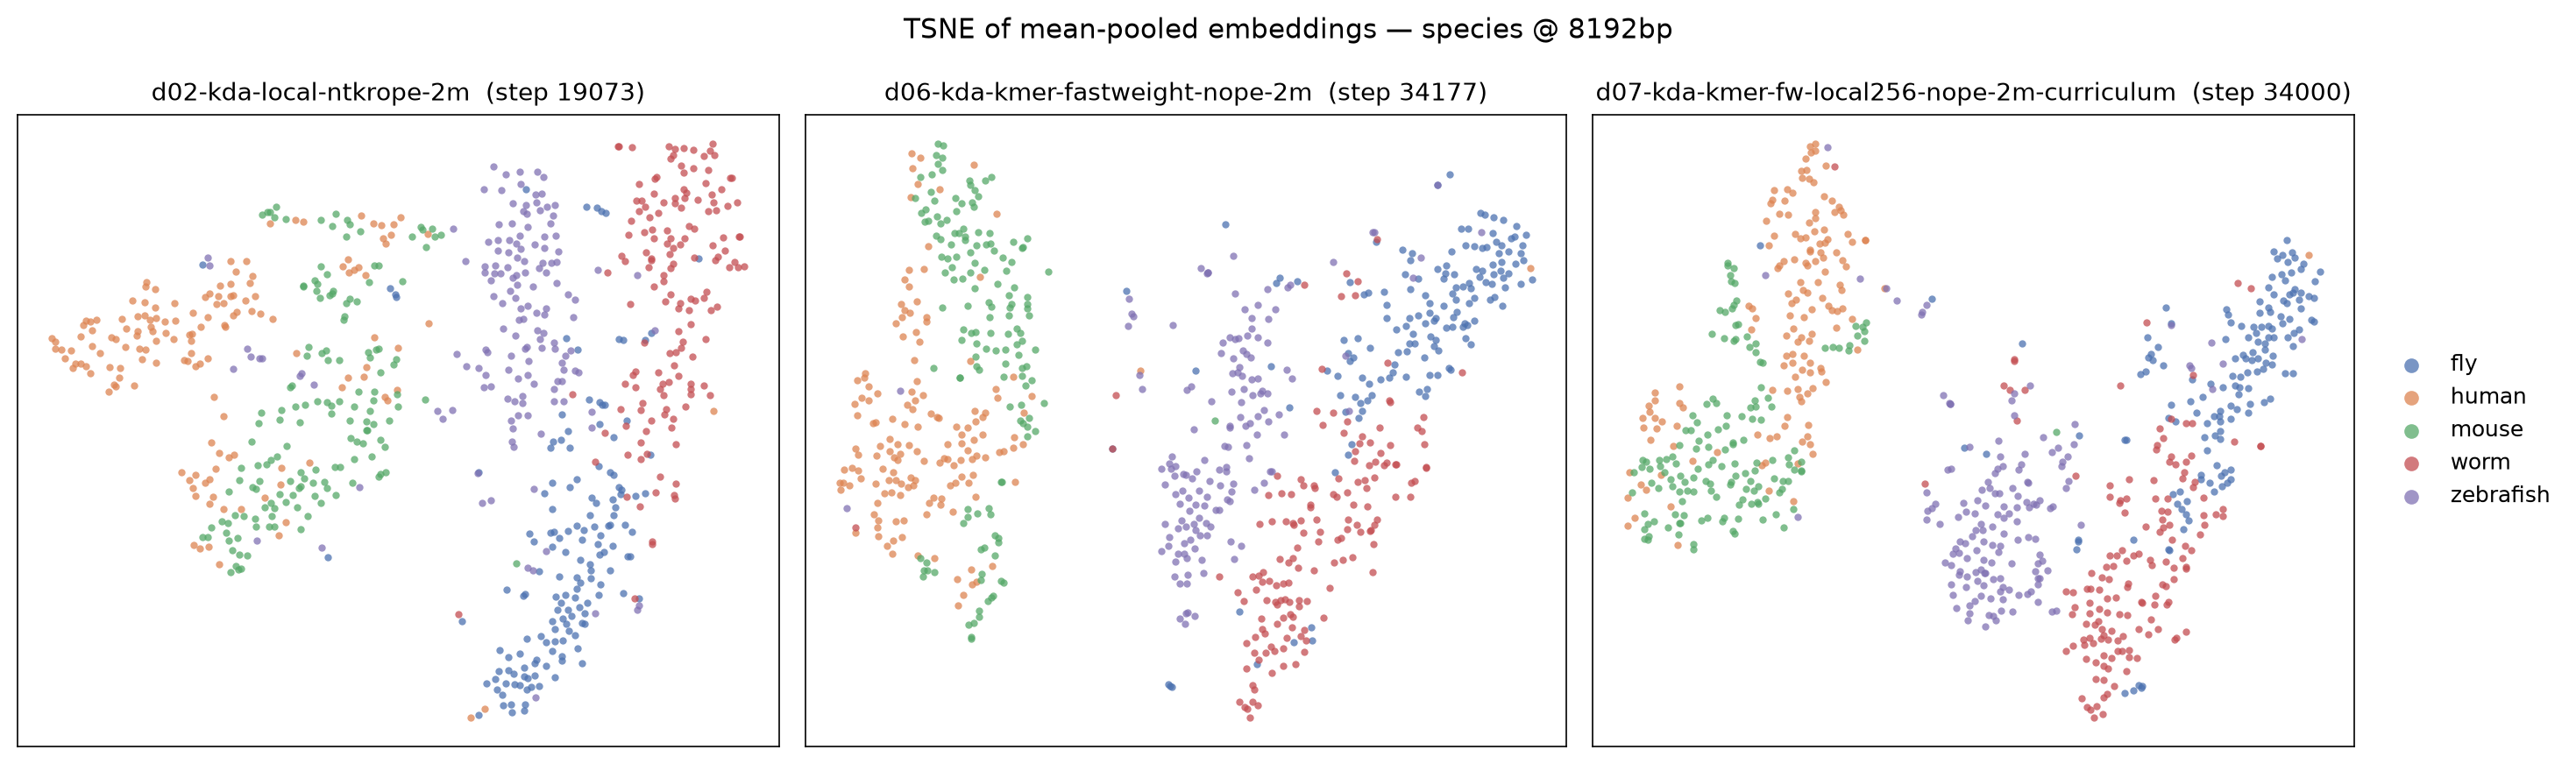
\includegraphics[width=\textwidth]{embed_tsne_species_8192_panel.png}
\caption{\textbf{t-SNE of mean-pooled embeddings} of 8{,}192\,bp genome windows from five species
(human/mouse/zebrafish/fly/worm), one panel per arm --- D02 (window-only), Mnemos-DNA, Mnemos-DNA-C --- all
pretrained on human sequence only. Species separate without any species supervision, and
vertebrates cluster together, mirroring phylogeny; this is the representation the frozen probe of
Figure~\ref{fig:species} reads out.}
\label{fig:tsne}
\end{figure}

\FloatBarrier
\subsection{Long-range regulatory and variant-effect prediction}\label{sec:exp-lrb}

\begin{table}[!tbp]
\centering\small
\resizebox{\textwidth}{!}{%
\begin{tabular}{lccccccc}
\toprule
Task (probe, 8\,K windows) & D01 & Mnemos-DNA & Mnemos-DNA-C & D02 & HyenaDNA-1M & Caduceus-PH & Caduceus-PS \\
\midrule
GLRB VEP eQTL (acc)      & 0.664 & \best{0.672} & 0.625 & 0.664 & 0.586 & 0.586 & \best{0.672} \\
GLRB enhancer (acc)      & 0.616 & 0.608 & 0.648 & \best{0.664} & 0.592 & 0.624 & 0.632 \\
GLRB promoter (acc)      & 0.942 & 0.942 & 0.942 & \best{0.950} & 0.934 & 0.934 & 0.934 \\
GLRB chromatin (mean acc)& --- & 0.931 & 0.937 & 0.929 & 0.933 & 0.937 & \best{0.938} \\
\bottomrule
\end{tabular}}
\caption{Genomics Long-Range Benchmark, frozen-backbone linear probes at 8\,K context, same
harness for every column; D01 is the matched pure-KDA control and D02 the window-only control of
Table~\ref{tab:arms}. A probe is a lower
bound on all models equally. External checkpoints (right three columns) are $\sim$3$\times$ our
parameter count and
pretrained with orders of magnitude more compute than ours; typical 95\% CIs span $\pm$0.07 on
eQTL/enhancer, so most differences here are individually indistinguishable --- the honest summary
is parity, reached at $\sim$2.3M parameters.}
\label{tab:lrb}
\end{table}

Table~\ref{tab:lrb} gives the frozen-probe results on the Genomics Long-Range
Benchmark~\cite{trop2024glrb} at 8\,K windows: at $\sim$2.3M parameters our arms sit at parity
with the external checkpoints on all four task groups, with most differences inside the
bootstrap intervals. The more interesting result is what happens when the window grows. Where
species identity rewards context, variant effect punishes it: every model degrades from 8\,K
to 32\,K windows on GLRB VEP eQTL (Mnemos-DNA: $0.672\to0.578$; Table~\ref{tab:lrb} reports the 8\,K
point). Diluting a SNP-centered signal with
context is not free. ``More context helps'' is a per-task question, and this is the task where the
answer is no --- worth stating in a paper whose efficiency story is about long windows.

\FloatBarrier
\subsection{GUE at the matched protocol, and a regression that dissolved}\label{sec:exp-gue}

\begin{figure}[!tbp]
\centering
\includegraphics[width=.85\textwidth]{fig_gue_delta.pdf}
\caption{\textbf{Per-task accuracy change on the 31-task GUE suite under the matched protocol}
(both arms: 4{,}000-example training cap, 6 epochs, bins$+$RC head, seed 0). The largest
per-task difference in either direction is $\pm$3.8 points and the suite means differ by 0.06
points --- the arms are equivalent on GUE. Under an unmatched protocol (differently sized
training sets on 28 of 31 tasks) the same checkpoints instead show a spurious $-5.3$-point mean
loss for Mnemos-DNA-C, dominated by the yeast \texttt{emp\_*} tasks.}
\label{fig:gue}
\end{figure}

\begin{table}[!tbp]
\centering\small
\begin{tabular}{lrrrrr}
\toprule
Suite (fine-tune, mean acc) & \#tasks & Pure-KDA (D01) & Mnemos-DNA & Mnemos-DNA-C & $\Delta$(C$-$M) \\
\midrule
Genomic Benchmarks~\cite{gresova2023genomic}        & 8  & 0.792 & \best{0.797} & 0.794 & $-0.3$ \\
Nucleotide Transformer subset~\cite{dallatorre2025nucleotide} & 6  & 0.787 & 0.793 & \best{0.794} & $+0.1$ \\
GUE (DNABERT-2)~\cite{zhou2024dnabert2}             & 31 & --- & \best{0.750} & 0.749 & $-0.1$ \\
\bottomrule
\end{tabular}
\caption{Suite-level mean fine-tuned accuracy under the matched protocol (Genomic Benchmarks and
Nucleotide Transformer means are over the seed means of Table~\ref{tab:downstream-abs}; GUE is
seed 0 for both arms; D01 was not run on GUE). GUE data is the
\texttt{leannmlindsey/GUE} HuggingFace community mirror of the DNABERT-2 release (the official
distribution cannot be fetched non-interactively), and should be cited as a community mirror.
Note the GUE means are not comparable to published DNABERT-2 numbers: the 4{,}000-example
training cap that makes the arms comparable to \emph{each other} also trains on far less data
than the official protocol on the larger tasks.}
\label{tab:suites}
\end{table}

Under the matched protocol the GUE ledger closes at zero: mean 0.750 (Mnemos-DNA) vs.\ 0.749
(Mnemos-DNA-C), with every per-task difference within $\pm$3.8 points (Figure~\ref{fig:gue},
Table~\ref{tab:suites}). The unmatched-protocol picture had suggested two further conclusions;
neither survives the matched rerun, and dissecting why is instructive.

\texttt{virus\_covid} --- under the unmatched protocol an alarming 0.657$\to$0.177 regression
that a learning-rate sweep could not recover --- is
explained: the 0.657 came from fine-tuning on the task's full 73{,}335-example training set,
the 0.177 from the 4{,}000-example cap. Under matched caps both arms sit at 0.166--0.177 on this
9-class task, barely above the 0.124 majority baseline, with near-maximal prediction entropy.
The correct statement is that \emph{neither} arm learns SARS-CoV-2 variant classification from
4{,}000 examples; the learning-rate sweep was probing a data-budget artifact. The
same applies to the \texttt{emp\_*} yeast epigenetic-mark ``degradation'': it tracked training-set
size, not architecture.

What survives is the dissociation: perplexity predicted none of this in either direction ---
the arms are 0.002 nats apart (\S\ref{sec:exp-lm}), appear 5--30 points apart per task under an
unmatched protocol, and are $\le$4 points apart under the matched one. Downstream deltas of
that size are within what \emph{evaluation protocol variation alone} produces, which
is itself this domain's restatement of ``perplexity is not capability'' --- and a caution about
how easily fine-tuned comparisons manufacture architecture stories.

\FloatBarrier
\subsection{Mechanism I: the recall bound}\label{sec:exp-recall}

\begin{figure}[!tbp]
\centering
\includegraphics[width=.9\textwidth]{fig_needle.pdf}
\caption{\textbf{Long-range exact recall (context 131{,}072).} A 256\,bp segment of real hg38
sequence is planted and the model must lower its loss when the segment repeats a distance $d$
later; the $y$-axis is the paired per-trial cross-entropy reduction versus a control (128
trials/point). The matched Pure-KDA control (D01) and the window-only hybrid (D02) are
indistinguishable from zero beyond 64\,bp. The $k$-mer
fast-weight arms hold 0.53--0.87 nats of advantage out to 64\,kbp, decaying smoothly with
distance.}
\label{fig:needle}
\end{figure}

The mechanistic result resolves cleanly (Figure~\ref{fig:needle}), and it now rests on a fully
matched control: D01 shares Mnemos-DNA's positional scheme (NoPE), training context, token
budget and data order, and differs only by the $k$-mer memory. Pure KDA's copy advantage is
$\approx$0.02 nats at distance 64 and zero beyond --- on genomic background it never performs
measurable exact recall at \emph{any} distance, so the finite-state recall bound is not a distant
cliff here but a wall at distance zero. The window-only arm D02, rerun in copy mode for this
figure, traces the pure-KDA curve point for point (0.016 at 64\,bp, zero beyond): windowed local
attention, despite exact token-level access inside its 512\,bp span, does not by itself convert
a repeated segment into a measurable copy advantage on hg38 background. The fast-weight memory
(Mnemos-DNA) recovers 0.87 nats at short
range and still holds 0.62 at 64\,kbp. Mnemos-DNA-C sits slightly below Mnemos-DNA at long distances (0.53 at
64\,kbp) --- the curriculum's short-sequence steps plausibly de-emphasize ultra-long carry ---
but the two memory arms are qualitatively identical. The memory, not the window, is what buys
recall.

\paragraph{The wall is a statement about this capacity, not about delta rules in general.} We
emphasize that the distance-zero wall is measured at edge scale: with
$d_{\text{model}}{=}128$ over 4 heads, each KDA head's state is a single $32\times32$ matrix ---
1{,}024 floats asked to summarize up to 131{,}072 tokens of genomic background, a regime where
sustained exact recall of an arbitrary planted segment is information-theoretically excluded long
before any architectural subtlety matters. State capacity grows quadratically in head dimension,
and larger delta-rule models on language do exhibit a graded recall-versus-distance profile
rather than a wall~\cite{arora2023zoology,yang2025gated}. The claim this section licenses is
therefore bounded: \emph{in the low-parameter edge regime, pure delta-rule recurrence cannot
sustain measurable exact recall on genomic background at any distance, and an auxiliary
decoupled memory --- here the $k$-mer fast-weight table --- is what restores it.} Whether a
scaled-up pure KDA closes the gap without such a memory is untested here.

The 0.82\,$\to$\,0.62 nat decay between 4\,kbp and 64\,kbp must be interference \emph{inside}
slot-level fast weights rather than address exhaustion, since address collision rates are
distance-independent (\S\ref{sec:method-capacity}) --- Proposition~\ref{prop:ema}'s EMA horizon is
the mechanism.

\paragraph{Degenerate motifs: the copy advantage survives point substitutions.} Because the
memory keys on \emph{exact} 8-mers, the natural objection is that biological motifs are
degenerate and a single SNP in a repeated segment could zero the mechanism out. We measured this
directly: the probe re-run with $m$ random point substitutions planted in the repeated 256\,bp
segment (\texttt{-{}-needle-copy-mutations}; sequence identity 99.6\% at $m{=}1$, 99.2\% at
$m{=}2$, 98.8\% at $m{=}3$), for both memory arms at the full 131{,}072 context
(Figure~\ref{fig:needlemut}). For Mnemos-DNA the copy advantage falls from 0.87 to 0.74 nats at
short range across $m{=}0\to3$ and from 0.62 to 0.51 at 64\,kbp; Mnemos-DNA-C behaves the same way
(0.84$\to$0.71 short range, 0.53$\to$0.44 at 64\,kbp). The cost is linear and small ---
$\approx$0.04 nats per substitution at short range, $\approx$0.03 at 64\,kbp, with no threshold
or collapse anywhere in the sweep --- and the curve shapes are unchanged, so the decay with
distance and the decay with divergence are independent. This is what the mechanism predicts: a
substitution invalidates only the $k{=}8$ addresses overlapping it ($\le 8$ of 249 addressed
positions per mutation), and at $m{=}3$ the remaining $\ge$90\% of the segment's 8-mers still hit
their slots. Exactness is required per \emph{address}, not per \emph{segment}.

\begin{figure}[!tbp]
\centering
\includegraphics[width=\textwidth]{fig_needle_mut.pdf}
\caption{\textbf{Recall under degenerate repeats} (context 131{,}072, 128 trials/point, shaded
95\% bootstrap bands). The repeat-copy probe of Figure~\ref{fig:needle} re-run with 0--3 random
point substitutions planted in the repeated 256\,bp segment, for Mnemos-DNA (left) and
Mnemos-DNA-C (right). Each substitution costs $\approx$0.03--0.05 nats roughly uniformly across
distances; the curves' shapes are unchanged, so the $k$-mer memory's recall is robust to
SNP-level divergence between repeat copies --- a substitution invalidates at most 8 of the
segment's 249 8-mer addresses. All curves, $m{=}0$ through $m{=}3$, are measured on the
main-suite checkpoints (step 34{,}177 for Mnemos-DNA, 33{,}900 for Mnemos-DNA-C).}
\label{fig:needlemut}
\end{figure}

\FloatBarrier
\subsection{Mechanism II: how the 65{,}536 slots are actually used}\label{sec:exp-slots}

\begin{table}[!tbp]
\centering\small
\begin{tabular}{lrr}
\toprule
Per 131{,}072\,bp held-out window (Mnemos-DNA, 8 windows) & Measured & Uniform-sequence null \\
\midrule
Addressed writes                              & 131{,}056 & 131{,}056 \\
Distinct slots written (of $4^8=65{,}536$)    & 41{,}342 (63.1\%) & 56{,}661 (86.5\%) \\
Colliding writes                              & 68.5\%   & 56.8\% \\
Writes per written slot (mean / p99 / max)    & 3.17 / 15 / 234 & 2.31 / 6 / --- \\
Effective slots $\exp(H)$ of the write distribution & 29{,}779 (45.4\%) & 56{,}661 \\
Share of writes in the top-20 slots           & 0.98\%   & --- \\
\ \ of which low-complexity (period $\le4$)   & 0.50\%   & --- \\
Mean write gate $g_w$, block 0 $\to$ block 6  & 0.226 $\to$ 0.865 & --- \\
\bottomrule
\end{tabular}
\caption{\textbf{Slot utilization on real hg38.} Addresses are a deterministic function of the
sequence, so the first five rows are identical across all 8 layers; only the write gate differs
by depth. Genomic non-uniformity costs capacity: 36.9\% of the address space is never touched in a
131\,kbp window, against 13.5\% under a uniform null, and the write distribution's effective
support is 45.4\% of the space. The most-written slot is poly-T (234 writes; poly-A is second at
138), but the repeat tail is \emph{narrow} --- the top 20 slots take under 1\% of all writes ---
so the capacity loss is broad non-uniformity, not a few repeat expansions. Deeper layers write
much harder than shallow ones, which under Proposition~\ref{prop:ema} means a shorter retention
horizon per slot near the output.}
\label{tab:slots}
\end{table}

Table~\ref{tab:slots} answers the capacity question empirically rather than from the pigeonhole
bound. Three things stand out. \emph{The space is under-used relative to its own null}: 63.1\% of
slots touched where uniform sequence would touch 86.5\%. \emph{Collisions are the norm}: 68.5\% of
writes land on an occupied slot, above the 56.8\% a uniform null predicts and well above the 50\%
pigeonhole floor --- which \S\ref{sec:method-capacity} argues is survivable, since a slot retains
up to 16 near-orthogonal key directions. And \emph{the popular intuition about repeats is only
half right}: poly-T and poly-A are indeed the top two slots by a wide margin, but the top 20 slots
together carry under 1\% of writes, so tandem repeats are not where the capacity goes. The
gradient in write-gate strength with depth (0.23 at block~0 to 0.87 at block~6) is a learned
division of labour --- early layers accumulate over many occurrences of an 8-mer, late layers
overwrite with the most recent one.

\FloatBarrier
\subsection{Mechanism III: which layer carries the splice-site signal}\label{sec:exp-layers}

This probe was designed to ask whether Mnemos-DNA-C's local-attention block exposes
splice-site structure --- the mechanism the unmatched-protocol numbers had appeared to demand
(\S\ref{sec:exp-snr}). The measurement stands on its own as a map of where splice-site
information lives in the stack, and it anticipated the correction: it found nothing special at
the window. We fit an independent
frozen linear probe on each of the 8 blocks' pooled representations (one embedding pass, identical
splits) on Nucleotide Transformer \texttt{splice\_sites\_all}:

\begin{center}\small
\begin{tabular}{lcccccccc}
\toprule
Block & 0 & 1 & 2 & 3 & \textbf{4 (local attn)} & 5 & 6 & 7 \\
\midrule
Probe accuracy & \best{0.689} & 0.687 & 0.666 & 0.654 & \textbf{0.653} & 0.668 & 0.673 & 0.672 \\
\bottomrule
\end{tabular}
\end{center}

\textbf{There is no separability jump at block~4 --- it is the worst block of the eight}, and
linear separability is highest at block~0 and declines through the middle of the stack. Read
alongside the matched fine-tuning result, the pieces now agree: the window exposes no emergent
linearly decodable splice-site structure, and under a matched protocol the fine-tuned numbers
show no repair for it to explain. The declining-with-depth profile is itself informative ---
splice-site information is most linearly accessible at the \emph{embedding-adjacent} blocks and
is progressively traded away through the stack, consistent with 131\,K-scale pretraining
allocating depth to long-range statistics at the expense of local grammar, which is the same
damage the random-init control exposes (\S\ref{sec:exp-snr}).

\FloatBarrier
\subsection{Deployment feasibility: memory and throughput}\label{sec:exp-deploy}

\begin{figure}[!tbp]
\centering
\includegraphics[width=.9\textwidth]{fig_scaling.pdf}
\caption{\textbf{Peak VRAM versus sequence length} (batch 1, bf16, single-sequence inference).
Mnemos-DNA(-C) inference is linear and reaches 1\,Mbp at 5.6\,GB; a full training step fits
through 256\,K. The released baselines' own batch-1 curves are shown directly: HyenaDNA-1M
reaches 256\,K (5.0\,GB) and goes out of memory at 512\,K; Caduceus-PS reaches 512\,K (7.6\,GB)
and goes out of memory at 1\,M. \textbf{This is a deployment-feasibility
comparison of released out-of-the-box checkpoints on consumer hardware}: the baselines
($\sim$3$\times$ our parameter count) run as shipped, without a
chunked path, while our 2.3M-parameter arms use a custom chunk-exact offload above 512\,K. It
measures what an 8\,GB deployment of these artifacts can open --- not an intrinsic sub-quadratic
advantage of KDA over Hyena or Mamba, which this experiment cannot establish.}
\label{fig:scaling}
\end{figure}

\begin{figure}[!tbp]
\centering
\includegraphics[width=.9\textwidth]{fig_throughput.pdf}
\caption{\textbf{Throughput is flat in sequence length}, as $O(N)$ requires: Mnemos-DNA(-C) prefill holds
250--350\,K\,tok/s from 8\,kbp to 1\,Mbp, and a full training step holds $\approx$70\,K\,tok/s.
Against the matched Pure-KDA control (D01, 400--720\,K\,tok/s) the $k$-mer table costs
$\approx$2$\times$ prefill throughput on top of its VRAM cost (Table~\ref{tab:footprint}) ---
a real constant-factor price, though one that leaves the length-scaling flat (a prior
comparison against the since-excluded D04 arm, whose inactive KV-cache path depressed its
throughput, had understated this cost; Appendix~\ref{sec:d04}).
Batch~1, bf16, one RTX~5060 (8\,GB).}
\label{fig:throughput}
\end{figure}

On the metric that matters for an edge deployment --- the longest single sequence processable at
all --- our arms reach 1\,Mbp at 5.6\,GB, where the released checkpoints stop at 256\,K
(HyenaDNA-1M and -450K, OOM at 512\,K) or 512\,K (Caduceus-PH at 5.0\,GB, Caduceus-PS at
7.6\,GB; both OOM at 1\,M) in the same harness on the same card;
Figure~\ref{fig:scaling} shows the batch-1 peak-VRAM curves, linear in length for every arm
shown. Throughput is flat in length, as $O(N)$ requires (Figure~\ref{fig:throughput}).

Measurement protocol matters here as much as in fine-tuning: a batched embedding pipeline (8
sequences at once) yields apparent baseline ceilings of 16--32\,K --- an 8$\times$
overstatement of the gap. All ceilings reported in this paper come from single-sequence
inference, the deployment-relevant measurement, under which our arms open windows
2--4$\times$ longer than the released baselines on this card.

Two honest qualifications remain. First, the comparison is between artifacts, not algorithms:
those checkpoints are $\sim$3$\times$ our parameters (HyenaDNA-1M 6.5M, Caduceus-PH/PS 7.7M),
are run as shipped without chunking, and were never intended for
an 8\,GB card, so the gap confounds model size, implementation and architecture. A
parameter-matched, chunking-matched comparison is a different experiment and we have not run it.
Second, the $k$-mer table makes our arms \emph{less} memory-light than pure KDA (D01 runs a
1\,Mbp forward in 5.5\,GB natively and needs no offload anywhere in the sweep; Mnemos-DNA(-C)
need the chunk-exact offload path above 512\,K), which
is the space cost of Table~\ref{tab:footprint} showing up in practice.

\FloatBarrier
\section{Discussion and Limitations}\label{sec:disc}

\paragraph{Protocol drift can manufacture architecture ``results,'' and we measured it doing
so.} Two apparent headline findings --- a $+30.4$-point splice repair and a $-5.3$-point
GUE cost --- arose during this study from comparing arms fine-tuned under different heads,
epoch budgets and training-set caps, protocol drift accumulated over months; both vanished
under the frozen matched protocol. We consider
quantifying this the most transferable finding in the paper: fine-tuned downstream comparisons
between architectures are fragile to exactly the kind of incremental protocol improvement
(a better pooling head, a longer budget) that gets applied to the newest arm first. Everything
downstream in this version runs under one frozen protocol, launched from a single queue script
that records the full command line per row.

\paragraph{The composite is not decomposed --- but it no longer needs to be.} Mnemos-DNA-C's two
changes were introduced together, so any Mnemos-DNA-C-specific effect belongs to the pair. Under
the matched protocol the pair's downstream effect is $\le$1 point on every suite mean, its
recall effect is a modest reduction at long range, and its LM effect is 0.002 nats; the
curriculum-only control is now of secondary interest, relevant mainly to whether short-context
validation parity (Figure~\ref{fig:curves}) can be had for free.

\paragraph{Seeds and intervals.} Fine-tuned numbers now carry 2--3 seeds per cell
(Table~\ref{tab:downstream-abs}); typical per-task seed spread is 0.2--2 points, which is why we
treat sub-2-point differences as unresolved even where bootstrap intervals are narrow.
Pretraining remains a single run per arm at one data order --- pretraining-seed variance is
unmeasured, and the bootstraps still cover split-sampling noise only. The large effects --- the
recall wall (0.6 nats), the random-init splice gap ($\sim$9 points), the OOM ceilings --- are
far outside both noise terms.

\paragraph{Exact recall is per address, not per segment.} The $4^8$ address space keys on exact
8-mers, and biology's motifs are degenerate --- the objection we expected to be sharpest. The
mutation sweep (\S\ref{sec:exp-recall}, Figure~\ref{fig:needlemut}) now bounds it for both memory
arms: up to three point substitutions in the repeated segment cost $\approx$0.04 nats each, linearly
and without a threshold, and do not change the shape of the recall curve. What remains open is
heavier divergence --- indels, rearrangements, and substitution rates high enough to break most
of the segment's 8-mers rather than a few percent of them.

\paragraph{Capacity ceiling at $d_{\text{model}}{=}128$.} Nucleotide Transformer
\texttt{promoter\_all} is pinned at 0.84--0.85 for every arm and for the random-init control
(GC content alone yields 0.81). At the edge-scale operating point this study targets, some
tasks are simply out of reach, and we report them as capacity ceilings rather than as architecture
comparisons.

\paragraph{Baseline comparisons are about artifacts.} The HyenaDNA/Caduceus columns share our
harness but not our model size ($\sim$3$\times$ ours), pretraining budget, or inference path.
Where they match or
beat us the reading is unremarkable; where we match them at 2.3M parameters the reading is
parameter efficiency; and their OOM ceilings describe 8\,GB deployment of those released
checkpoints, not the methods at their native scale --- measured at batch 1, after we corrected
an earlier probe-batch confound that had overstated the gap 8-fold (\S\ref{sec:exp-deploy}).

\paragraph{What we would test next.} An intervention that actually closes the splice-site gap to
random init --- the window-plus-curriculum patch did not, so the candidates are shorter or mixed
pretraining lengths from step 0, or a pretraining objective term that protects local grammar;
the remainder of the mutation
sweep (indels and rearrangements); a window-size sweep of the local layer; a bf16 fast-weight table to halve
the 512\,MiB inference state; and a variable $k$ (or a learned address function) to attack the
36.9\% of address space that hg38 never touches.

\section{Conclusion}\label{sec:conc}

Gated delta-rule linear attention is a workable base operator for character-level genomic modeling
at edge scale --- but not alone. At this operating point's state capacity, pure KDA's
finite-state recall bound is not a distant cliff on DNA; it is a wall at distance zero, and a
windowed local-attention layer does not move it. A
content-addressed $k$-mer fast-weight memory removes most of that wall --- robustly to SNP-level
divergence in the repeated material --- for $\sim$3\% extra parameters, a $\approx$2$\times$
prefill-throughput constant, and a 4096$\times$ larger recurrent state, while preserving $O(N)$
scaling and megabase-length exact chunked inference on an 8\,GB GPU; all three costs are
accounted for rather than omitted. Its address space is used
unevenly: two thirds of slots touched in a 131\,kbp window, 68.5\% of writes colliding, and a
delta rule inside each slot that turns those collisions into a gated regression rather than a
clobber. The fixed ultra-long pretraining context that makes such models impressive at length
makes them \emph{worse} at sub-kilobase grammar than their own random initialization --- a
failure our window-plus-curriculum patch did \emph{not} repair, and which stands as the study's
sharpest open problem. And fine-tuned downstream comparisons proved protocol-fragile: apparent
30-point architecture effects arise from head, budget and data-cap drift alone and vanish under
one matched fine-tuning protocol, which we report as a result in its own right: at this scale,
evaluation-protocol drift can produce larger architecture ``effects'' than architecture does.
The trade-offs, not the wins, are the finding: recall, context length, and short-range grammar
are three different budgets, and an architecture choice that spends one is spending it from
somewhere.

\appendix

\section{Pre-registered hypotheses and verdicts}\label{sec:hyp}

The following hypotheses were stated in the study plan before the Mnemos-DNA(-C) comparison was run, so
that outcomes could not be reframed after the fact. Each carries an explicit falsifier.

\begin{hypothesis}[Deployment efficiency; high prior confidence]\label{hyp:eff}
Under a fixed 8\,GB VRAM ceiling, the $O(N)$ KDA arms will process strictly longer sequences than
the released convolutional and SSM checkpoints, with peak memory growing linearly in sequence
length. \emph{Falsifier:} any baseline matching or exceeding the KDA arms' maximum feasible
context on the same card. \emph{Test:} \S\ref{sec:exp-deploy}.
\end{hypothesis}

\begin{hypothesis}[Recall bound]\label{hyp:recall}
Pure KDA's exact-recall accuracy will degrade past a distance threshold set by its finite state
capacity; the $k$-mer fast-weight memory, which factors exact 8-mer recall out of that state,
will hold up at longer range; a windowed local layer adds exact recall only inside its
$\sim$256--511\,bp span. \emph{Falsifier:} pure KDA matching the memory-augmented arms at long
range, or the memory arms degrading identically to pure KDA. \emph{Test:} \S\ref{sec:exp-recall}.
\end{hypothesis}

\begin{hypothesis}[Language-model loss; no prior stated]\label{hyp:ppl}
Pretraining perplexity across arms was pre-registered as genuinely uncertain, with no directional
expectation. \emph{Test:} \S\ref{sec:exp-lm}.
\end{hypothesis}

\begin{hypothesis}[Downstream capability; dissociation expected]\label{hyp:down}
Downstream fine-tuned accuracy was pre-registered as uncertain, with the explicit caution that
perplexity may not predict it. A Mnemos-DNA-C-specific sub-hypothesis, formed after observing Mnemos-DNA's
splice-site failure and before Mnemos-DNA-C was trained: a local-attention window plus a length curriculum
will repair sub-kilobase position-sensitive tasks that fixed-131\,K pretraining damaged.
\emph{Falsifier:} Mnemos-DNA-C failing to close the gap to the random-initialization control on splice
sites. \emph{Test:} \S\ref{sec:exp-snr}.
\end{hypothesis}

\begin{table}[h]
\centering\small
\begin{tabular}{p{2.0cm}p{4.3cm}p{3.4cm}p{4.3cm}}
\toprule
Hypothesis & Pre-registered prediction & Verdict & Evidence \\
\midrule
H\ref{hyp:eff} deployment efficiency & KDA arms exceed released baselines' max context on 8\,GB &
\best{Supported}, with a shrunk margin & 1\,Mbp vs.\ 256\,K--512\,K before OOM at batch 1
(Figs.~\ref{fig:scaling},~\ref{fig:species}); an earlier 32\,K/16\,K figure was a probe-batch
confound; confounds model size ($\sim$3$\times$) \\
H\ref{hyp:recall} recall bound & Pure KDA degrades past a distance threshold; memory arms hold
longer; a local window adds recall only inside its span & Supported, stronger than predicted &
Matched pure KDA (D01) has \emph{no} recall at any distance and the window-only arm (D02) is
identical to it; memory arms hold to 64\,kbp (Fig.~\ref{fig:needle}), robustly to 1--3
substitutions (Fig.~\ref{fig:needlemut}) \\
H\ref{hyp:ppl} LM loss & No direction stated & Parity & All arms within 0.01 nats; flat
8\,K--1\,M (Figs.~\ref{fig:curves},~\ref{fig:lmctx}) \\
H\ref{hyp:down} downstream & Perplexity--capability dissociation; window+curriculum repairs
sub-kb tasks & Dissociation supported; \textbf{repair sub-hypothesis falsified} & Under the
matched protocol Mnemos-DNA-C does not close the gap to the random-init control on splice sites
(0.733 vs.\ 0.832), so the stated falsifier fired. An earlier apparent $+30.4$-point repair was
a fine-tuning-protocol artifact (\S\ref{sec:exp-snr}); the GUE regression reported alongside it
dissolved under the same audit \\
\bottomrule
\end{tabular}
\caption{Verdicts on the pre-registered hypotheses. ``Supported'' means the falsifier stated above
did not occur --- not that the proposed mechanism is confirmed. H\ref{hyp:down}'s repair
sub-hypothesis is the study's one falsified prediction, and it was briefly ``supported'' by
numbers that a protocol audit later invalidated --- the sequence of events \S\ref{sec:disc}
argues is itself worth reporting.}
\label{tab:verdicts}
\end{table}

\section{The excluded D04 arm, and a bf16 cautionary note}\label{sec:d04}

Earlier drafts used an arm labelled D04 as the pure-KDA control. An audit found that D04 was in
fact a KDA variant with an auxiliary evicted-KV exact cache whose 32 scalar cache gates, stored
in bf16, sat at \emph{exactly} their $-4.0$ initialization (sigmoid $= 0.018$) after the full
5.0B-token run: bf16's rounding granularity around small gradient updates froze them, so the
cache path was inactive for the entire run while still costing throughput (its 80--98\,K\,tok/s
was the source of a prior, incorrect ``the $k$-mer table is throughput-free'' comparison).
D04 was excluded and replaced by D01, a true pure-KDA arm trained under the fully matched
protocol (NoPE, 131\,K context, 4.5B tokens, same data order). The general lesson is the one
already noted in \S\ref{sec:method-d06}: scalar gate parameters must be kept in fp32; every arm
in this paper does so, and any arm trained before that fix should have its gate parameters
checked against their initialization before its numbers are trusted.

\bibliographystyle{unsrt}
\bibliography{refs}

\end{document}
